\subsection{Euclidean distances analysis for Zernike modes PSFs with a 42 waveguide PL}

	\subsubsection{Preprocessing}
		
		\begin{itemize}
			\item The PSF electric fields matrices are flattened to compute the euclidean distances between 1d vectors.
			\item 70000 datapoint pairs for each zernike datasets are randomly defined. The euclidean distances will be calculated for these selected pairs.
			\item In this case, LP coefficients are also analysed.
		\end{itemize}
			
	\subsubsection{Results}
		\begin{figure*}[ht!]
			\centering
			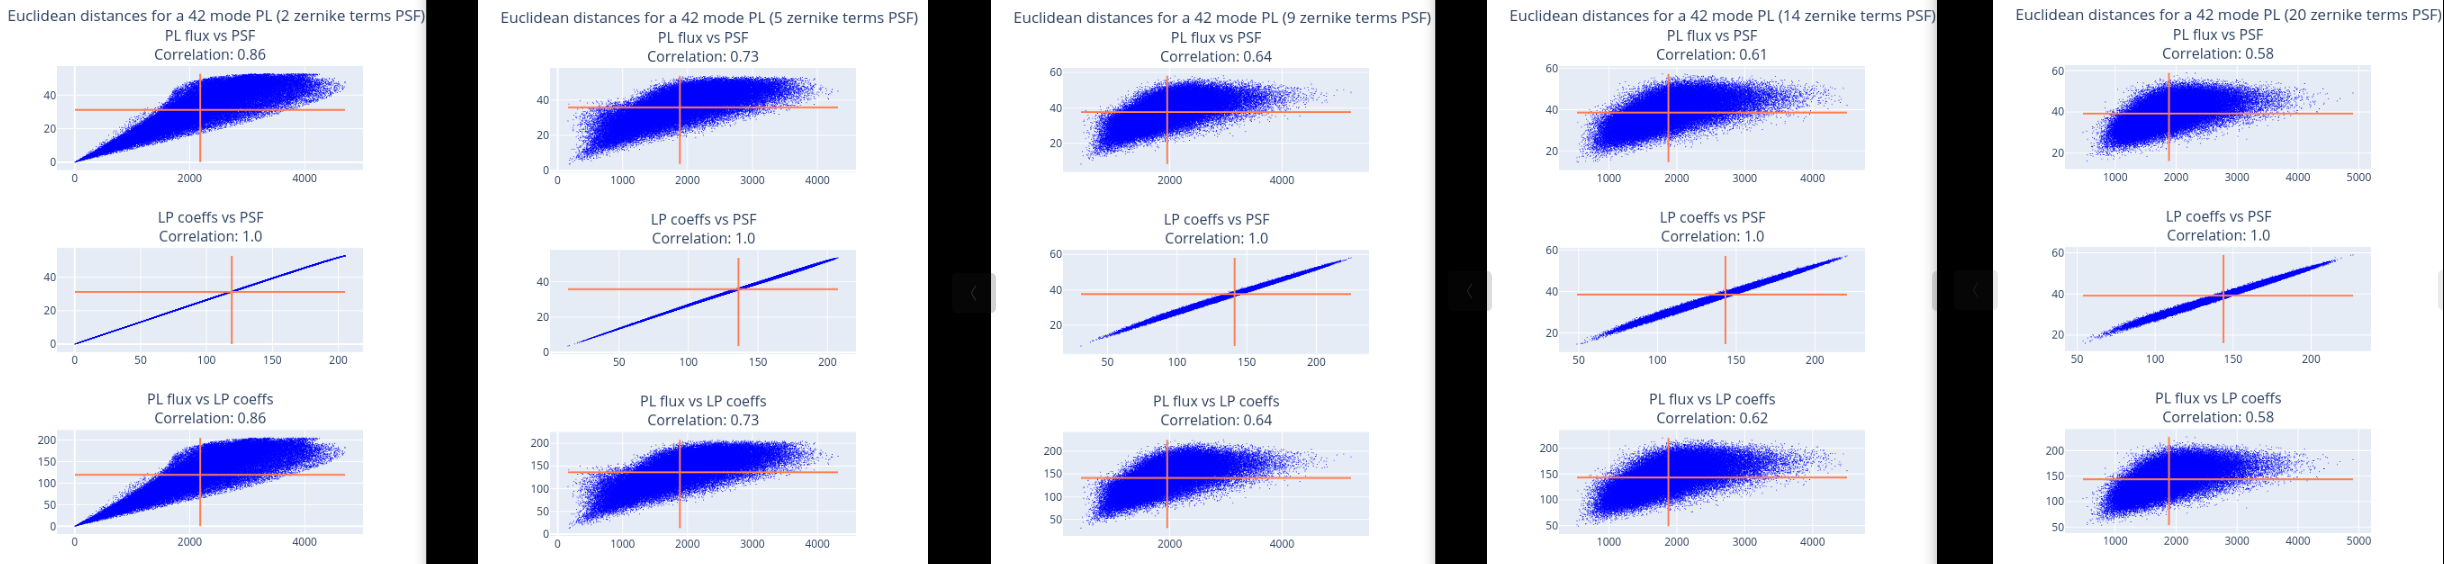
\includegraphics[scale=0.22]{pid-euclideandistanceszernike42pl.png}
			\caption{Euclidean distances relationship between the Zernike PSFs datasets}
		\end{figure*}
    
    
     
		\FloatBarrier